\documentclass[tcn = 37075, sheet = true, abstract = true]{mcmthesis}
\problem{A}
\usepackage{palatino}
\usepackage{mwe}
\usepackage{slashbox}
\usepackage{algorithm2e}
\usepackage{mathrsfs}

\title{Understanding Employee Churn based on Information Accumulation and Bayesian Learning}
\author{\small \href{http://www.latexstudio.net/}
  {
\includegraphics[width=7cm]{mcmthesis-logo}}}
\date{\today}

\begin{document}
\begin{abstract}
\lipsum[1]
\begin{keywords}
keyword1; keyword2
\end{keywords}
\end{abstract}
\maketitle
\newpage


\tableofcontents
\newpage
\section{Introduction}

\section{Setting up the Background}

(\textit{This paragraph needs rephrasing later}) Building the organizing network of the company requires first to plausibly incorporating the organizational graph (as presented in figure 1) and the allocation of different levels of positions (as indicated in table 1). To reach this, we assign different positions to different offices according to several rules. After some minor adjustments, we can get a possible and reasonable allocation of staff, on which we will build our later analysis. The assumptions related to the allocation are as follows:

\noindent \textbf{Assumptions}:

To explain the assumptions clearly, we first define terms "tree" and "tier". Tree is defined to be the whole picture of the organizational graph. Entries are defined to be in the same tier if they are on the same horizontal line in figure 1. Thus we can see that the tree stems from the higher tier of CEO to the lowest tier of branches. Now the assumptions:

\begin{itemize}
\item Every senior/junior manager should have a clerk in his/her office for administrative tasks.
\item The level of position of a staff tend to be higher when his office is closer to the CEO in the organizational graph.
\item The level of position of a staff tend to be higher when his office is the root of divisions of more people.
\item The level of position of a manager cannot be lower than someone whose office belongs to a lower tier.
\item Research tasks should be conducted by experienced employees.
\end{itemize}

Thus we can get the following table of allocation of 370 positions:
\begin{table}[htb!]
\centering
\begin{tabular}{l|lllllllll}   \hline
\backslashbox{Tier}{}& \backslashbox{Position}{level}&1&2&3&4&5&6&7&Total\\ \hline
1                  & CEO              & 2              & 0              & 0                      & 0                        & 0                    & 0                      & 2                    & 4     \\
\multirow{7}{2pt}{2} & Research           & 1              & 0              & 0                      & 0                        & 2                    & 0                      & 1                    & 4     \\
                   & CIO                & 1              & 2              & 0                      & 0                        & 8                    & 0                      & 3                    & 14    \\
                   & CFO                & 1              & 2              & 0                      & 0                        & 8                    & 0                      & 3                    & 14    \\
                   & HR                 & 0              & 1              & 0                      & 0                        & 2                    & 0                      & 1                    & 4     \\
                   & VP                 & 2              & 0              & 0                      & 0                        & 0                    & 0                      & 2                    & 4     \\
                   & Facilities         & 1              & 0              & 0                      & 0                        & 2                    & 0                      & 1                    & 4     \\
                   & Sales Marketing    & 1              & 0              & 0                      & 0                        & 2                    & 0                      & 1                    & 4     \\
 \multirow{9}{2pt}{3} & Networks           & 0              & 1              & 1                      & 0                        & 11                   & 0                      & 1                    & 14    \\
                   & Information        & 0              & 1              & 1                      & 0                        & 11                   & 0                      & 1                    & 14    \\
                   & Program Manager    & 0              & 1              & 1                      & 0                        & 6                    & 5                      & 1                    & 14    \\
                   & Production Manager & 1              & 1              & 0                      & 0                        & 10                   & 0                      & 2                    & 14    \\
                   & Plant Blue         & 0              & 1              & 1                      & 0                        & 6                    & 5                      & 1                    & 14    \\
                   & Plant Green        & 0              & 1              & 1                      & 0                        & 6                    & 5                      & 1                    & 14    \\
                   & Regional           & 0              & 1              & 1                      & 0                        & 6                    & 5                      & 1                    & 14    \\
                   & World Wide         & 0              & 1              & 1                      & 0                        & 6                    & 5                      & 1                    & 14    \\
                   & Internet           & 0              & 1              & 1                      & 0                        & 6                    & 5                      & 1                    & 14    \\
4                  & Director           & 0              & 6              & 6                      & 0                        & 6                    & 0                      & 6                    & 24    \\
5                  & Branch             & 0              & 0              & 11                     & 25                       & 12                   & 120                    & 0                    & 168   \\ \hline

&Total              & 10             & 20             & 25                     & 25                       & 110                  & 150                    & 30                   & 370 \\  \hline
\end{tabular} 

*1:Senior Manager 2:Junior Manager 3:Experienced Supervisor 4:Inexperienced Supervisor 5:Experienced Employee 6:Inexperienced Employee 7:Administrative Clerk

\caption{The distribution of staff in different positions}
\end{table}



We set up to build the network in this company. Define $V(G)=\{v_1,v_2,...v_{370}\}$ as the set of all positions. Each node denotes one position. Define $E(G)$ is the set of edges in the network. $(v_i,v_j)\in E(G)$ if at least one of the following holds:


\begin{itemize}
\item $i$ and $j$ are in the same office. Here one entry in figure 1 is considered as an office, whether it consists of two divisions of 14 staff members or only four staff members.
\item $i$ is the head of an office and $j$ is the head of the directly-related upper office or the opposite. Here the staff member in the highest level of position within an office is considered as the head of the office, such as the junior manager in Networks office and the experienced supervisor in Branch office.
\item $i$ and $j$ are both senior manager or junior manager.
\end{itemize}

$G=\{V(G),E(G)\}$ is the the graph of this network. We then visualize the network in the following picture (figure 1).

\textbf{input the Gephi graph}

\begin{figure}[htb!]
\small
\centering
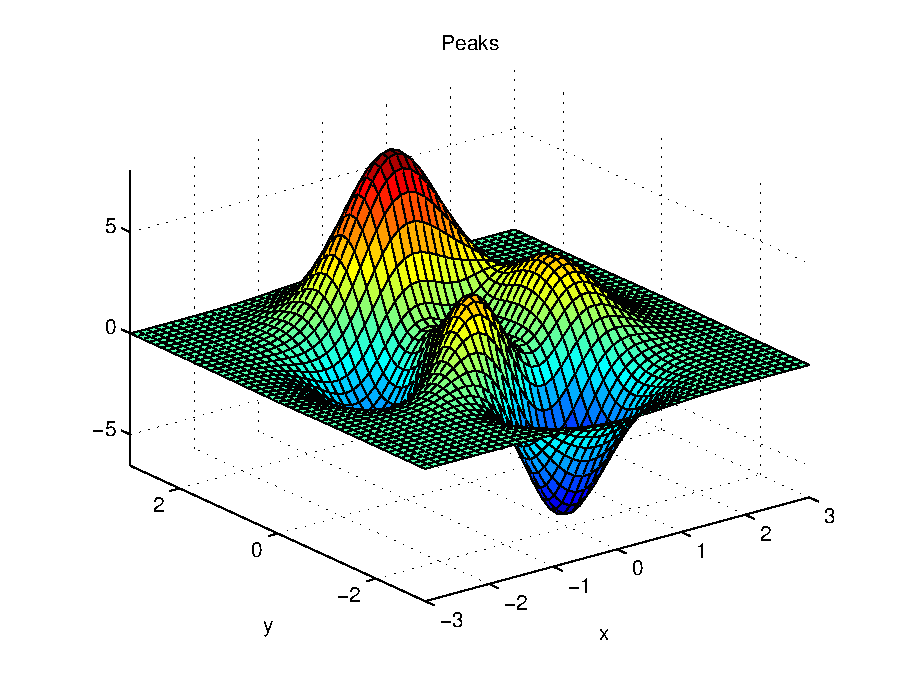
\includegraphics[width=12cm]{mcmthesis-aaa.eps}
\caption{aa} \label{fig:aa}
\end{figure}

Then we turn to the main part of building up our model and using it for analysis. To deal with the complicated real problems, we first simplify them into two process. The first process is named as "output" and the second process is named "input". Like in the real world and in the problem, the "output" process refers to the situations where the staff leave his or her position. The "input" process, accordingly, refers to the combination of internal promotion and outsourcing recruitment. The formal models are presented in the next section. Based on this process division, we can easily see that the "input" process is where the Human Resource manager works his or her power to control and improve the company's current position.


\section{Models}

We hold the intention to create a dynamic model which can be controlled by manipulating some of the parameters. Specially, we assume that the "output" process is largely determined by individual characteristics rather than company's policy. However, we also want to create a set of tools that human resource managers can use to deal with the possible staff problems. With these in mind, we design two models that capture the process of "output" with different emphasis and simulate three possible strategy for the human resource manager: purely recruiting, purely promoting and the "greedy" strategy. These models and simulations will help to solve the task 1-5 and even dig deeper insights about staff management. 

We made some assumption concerning the timeline of our model:
\begin{itemize}
\item We use one month as our minimum time interval.
\item New employees start working at the beginning of the month and resigned employees end their work at the end of the month.
\end{itemize}

To begin with, we give some definitions: 
\begin{itemize}
\item $\Gamma^{(t)}$: the set of people who work in the company at the beginning of period $t$ after recruitment.
\item $\Omega^{(t)}$: the set of people who leave the company at the end of $t$. \item $\Theta^{(t)}$: the set of people who enters the company at the beginning of $t$. 
\item $f^{(t)}$: the mapping from $\Gamma^{(t)}$ to $V(G)$, which maps individual $i\in \Gamma^{(t)}$ to his position $f^{(t)}(i) \in V(G)$ at time $t$.
\end{itemize}

It's obvious that the relation $\Gamma^{(t+1)}=\Gamma^{(t)}\bigcup \Theta ^{(t+1)} \backslash \Omega^{(t)}$ holds.

Next we begin to build the model from two aspects: "output", which means the resign of current staff, and "input", which means the recruitment of new staff.

\subsection{Understanding "Output"}

\subsubsection{Model I : Capture Churn Using Information Accumulation}

\paragraph{Information Effect}
In this model, we capture the way an individual is influenced by other people's leaving using information flow. In other words, the event of one person leaves acts as a influential message, transmitting across the network built earlier. We call it information effect. We assume that the information effect will accumulate, that is, the churn news this month and last month will have an equal and add-up influence in shaping the listen's decision. In order to make the model easier to control, we add an assumption that the a piece of information's effect will expire after six months. This modeling technique can be justified by the psychological evidence (\textbf{where to find any???}) that . 

To formalize this process in mathematical expressions, we first define some metric to measure the information effect. 

\begin{itemize}
\item Influence: The resign of staff in different level of position has different influence on other people. We denote the influence by $e^{(t)}_i,i\in \Gamma^{(t)}$. We further assume influence is the same for individuals in the same level of position.
\item Distance: The distance between two nodes $i$ and $j$, $d(i,j)$ is defined by the length of the shortest path connecting $i$ and $j$ in the graph. For two individuals in the company, We define the distance between $i, j\in  \Gamma^{(t)}$, $d_{ij}^{(t)}$, by $d(f^{(t)}(i),f^{(t)}(j))$.
\item Information effect is proportional to the influence.
\item Information effect is inversely proportional to the squared distance.
\item Information effect is accumulated for the past six months.
\end{itemize}

Formally, the information effect on individual $i\in \Gamma{(t)}$ can be calculated as follows:

$$\displaystyle \sum_{\tau=t-6}^{t-1}\sum_{j\in \Omega^{(\tau)}}\frac{e_j^{(\tau)}}{d_{ij}^{(\tau)2}}$$

\paragraph{Tenure Effect}

Another aspect we take into consideration is called tenure effect. \textbf{where to find any???} The longer an individual stays in the same position, the more likely he/she is to be dissatisfied with his current condition. We add a multiplier before the information effect to incorporate this additional effect. Besides, tenure effect tend to increase faster as tenure increases. So we simply adopt the quadratic form.

Combine information effect and tenure effect, we develop a measure called "dissatisfaction" $\sigma_i^{(t)}$:

$$\displaystyle \sigma_i^{(t)}=(1+kt_i^{(t)2})*\sum_{\tau=t-6}^{t-1}\sum_{j\in \Omega^{(\tau)}}\frac{e_j^{(\tau)}}{d_{ij}^{(\tau)2}}~~~~\forall i\in \Gamma{(t)}$$

Here $t_i^{(t)}$ is the length of individual $i$ has stayed in his current position at time $t$ and $k$ is the control parameter. 

\paragraph{Tolerance Threshold}

For each individual, he has an internal tolerant threshold $\zeta_i$. When his dissatisfaction measure exceeds his threshold and he is not promoted, he will decide to leave this company. Tolerant threshold is not necessarily a fixed value. We assume it is uniformly distributed in the interval $\displaystyle [m_i-\frac{1}{2\alpha m_i},m_i+\frac{1}{2\alpha m_i}]$. We further assume common middle point $m_i$ for all individuals in the same level of position.


\subsubsection{Model II : Capture Churn Using Bayesian Learning}

% Another way of capturing the effect from others can is to interpreted it as a learning process, which is widely discussed in network science and economics literature (\textbf{to be precise???}Jackson 2013; Acemoglu 2008;). The main context for this kind of modeling lies in that individuals perceives two states of the world or actions and act in response based on Bayesian inference. In the settings of this problem, this two states are \textit{to leave} or \textit{to stay}.

In recent studies, Bayesian learning has been used to analyze information aggregation in social networks, in which individuals modify their decision based on previous outcomes of other individuals in the network. (A cite is needed for the topic Bayesian Learning in Social Networks)

We introduce a novel method to model the churn rate based on Bayesian learning methods. Specifically, we view the churn as a decision making process: suppose an individual $i$ decides whether to churn in a particular month $m$ based on a random variable $u_{i,t} \in \{0, 1\}$, where $u_{i,t} = 0$ indicates a churn, otherwise a non-churn is indicated. $u_{i, m}$ is drawn as follows:
\begin{enumerate}
\item Assume two hyperparameters $\alpha_{i, t}$ and $\beta_{i, t}$;
\item Draw 
  \begin{equation}
   p_{i, m} \sim \mathrm{Beta}(\alpha_{i, t}, \beta_{i, t})
   \label{eq:beta}
  \end{equation}
  where $\displaystyle \mathrm{Beta}(x; \alpha, \beta) = \frac{x^{\alpha - 1}(1-x)^{\beta - 1}}{\mathrm{B}(\alpha, \beta)}$, and $\mathrm{B}(\alpha, \beta)$ is the normalization constant.
\item Draw 
  \begin{equation}
	u_{i, t} \sim \mathrm{Bernoulli}(p_{i, t})
    \label{eq:bernoulli}
  \end{equation}
  where $\mathrm{Bernoulli}(x; p) = p^x(1-p)^{1-x}$ is the Bernoulli distribution.
\end{enumerate}

The distribution of $u_{i, t}$ is a specification of the Beta-Binomial distribution, which has mean $\displaystyle \frac{\alpha}{\alpha + \beta}$ and variance $\displaystyle\frac{\alpha\beta}{(\alpha+\beta)^2}$. This distribution has good properties: on the one hand, the overall churn rate can be easily estimated using the hyperparameters of each individual; on the other hand, since the Beta distribution is the conjugate prior of the Bernoulli distribution, $\alpha$ and $\beta$ can be conveniently updated given observed results. For simplicity, please refer to Pattern Recognition and Machine Learning for more details.

Updating the hyperparameters $\alpha$ and $\beta$ can be viewed as a Bayesian learning process: an increase in $\alpha_i$ decreases $i$'s tendency to churn, while an increase in $\beta_i$ increases this tendency. Moreover, increasing $\alpha_i$ and $\beta_i$ reduces the variance of the Beta distribution, indicating that the individual has a better estimation of $p_i$. We also take the network structure into account, where the outcome of nearer individuals have more influence.

The update process is described in Algorithm \ref{algo:bayes}:

\RestyleAlgo{boxed}
\begin{algorithm}[H]
 \KwData{The network $G$, and the churned individuals in the first month $\Omega^{(t)}$}

 initialize t = 0, $\alpha_{i,0}$ and $\beta_{i,0}$ for $\forall i \in \Gamma(t)$\;
 \While{True}{
   \For{$\forall i \in \Gamma(t) \backslash \Omega^{(t)}$}{
   	 $\hat{\alpha} = \hat{\beta} = 0$\;
     \For {$\forall j \in \Gamma(t) \backslash \Omega^{(t)}$} {
     	$\hat{\alpha} = \hat{\alpha} + 1 / d_{ij}^{(\tau)2}$\;
     }
     \For{$\forall j \in \Omega^{(t)}$} {
        $\hat{\beta} = \hat{\beta} + 1 / d_{ij}^{(\tau)2}$\;
     }
     
     $\alpha_i = \alpha_i + \frac{\hat{\alpha}}{\hat{\alpha} + \hat{\beta}}$\;
     $\beta_i = \beta_i + \frac{\hat{\beta}}{\hat{\alpha} + \hat{\beta}}$\;
   }
   $\Omega^{(t)} = \Phi$\;
   \For{$\forall i \in \Gamma(t)$} {
     Sample $u_{i,t}$ according to \ref{eq:beta} and \ref{eq:bernoulli}\;
     \eIf {$u_{i, t} = 0$} {
       $i$ choose to churn\;
       $\Omega^{(t+1)} = \Omega^{(t+1)} \and \{i\}$;
     }{
     	$i$ choose not to churn\;
     }
   }
   $t = t + 1$\;
 }
 \caption{Algorithm for the Bayesian Churn Model}
 \label{algo:bayes}
\end{algorithm}

\subsection{Understanding "Input"}

In this part, we combine two parts that a HR manager can control, namely supplement strategies and experience requirements, to define the "input" in our model. To be more specific, supplement strategies here are the schemes of both promotions and recruitment. They are combinedly referred to as "supplement strategy". The experience requirements refer to the needed length of being in one position before getting promoted.

\subsubsection{Supplement Strategies}

(\textit{This paragraph needs refinement later}) Two most easily named strategies are purely promoting strategy and purely recruiting strategy. We will see what these strategies lead us to in the next section. Besides these two simple strategies, we also have a strategy called "greedy" strategy in our paper. This "greedy" strategy is most efficient among all the relatively simple strategies, which we will prove later.(\text{!!!!!!!!!!!!!!!!!!!!!!!!!!}) Therefore it is the main focus of our simulations. We will also base most of our numeric results on it.

The scheme for this "greedy" strategy can be described by the following rules:
\begin{itemize}
\item When there is a vacancy in the position, the HR manager will first rearrange the staff within the same tier to get a better \textbf{\Large{matching}}.
\item After this rearrangement, this strategy requires the HR manager to first seek opportunity to make promotions. The main reason is that promotion will save both the time and money needed for recruitment. However, any person getting promotion must first meet the experience requirement.
\item The above rule will not be obeyed for the situation where an inexperienced employee position is vacant. For recruiting a clerk costs more than recruiting an inexperienced employee directly.
\item \textit{The total number of recruitment is less than 37 (10\% of the total number 370 as mentioned in the tasks).}(\textbf{argued})
\item The recruitment will start only after observing a position is vacant and no person can be promoted to fill the vacancy. That is to say, the HR manager is "discreet". He doesn't believe in any prediction of the possible job vacancy under this strategy. In the meanwhile, he will place job vacancy in the higher level in higher order when considering recruiting. In other words, because of the upper limit of the total recruitment, there might be situations where vacant positions needing recruiting cannot be satisfied all. Then he will place the preceding order. The main consideration behind this lies in the recruitment time for higher tier is usually higher.
\end{itemize}

As we can see, supplement strategy effectively control the matching problem. Consider the company has been operating under this strategy for an enough long period of time, the friction will be all eliminated by this strategy because of the first step. \textbf{The proof:} \\

\subsubsection{Experience Requirement}

Both in reality and in the context of this problem, a certain amount of experience is required for getting promotion. Usually, the higher tier to be promoted into, the longer the experience is needed. In the model, we assume that the required experience for promotion only takes into account the time length of being in the former level. E.g. only the time length of being in the level of junior manager set to be requirement for consideration of promoting senior manager. Suppose the experience requirement for each level of position is represented by $R_i, i = 1, 2...,7$. This can be a rich set of tools that the HR manager can use to control the organizational structure and even churn rate.

\section{Estimation and Simulation}

\subsection{MLE Estimation of the Parameters in Model 1}

In this part, we briefly discuss how to estimate the parameter in Model 1 if we have additional information.

The unknown parameters are: the influence of different levels of position $e_i$ in the network $e_i$, the parameters depicting the distribution of tolerant threshold in different levels of position $m_i$ and $\alpha$ and the control parameter $k$ in tenure effect.

At time $t$, individual $i$ has dissatisfaction measure:

$$\displaystyle \sigma_i^{(t)}=(1+kt_i^{(t)2})*\sum_{\tau=t-6}^{t-1}\sum_{j\in \Omega^{(\tau)}}\frac{e_j^{(\tau)}}{d_{ij}^{(\tau)2}}~~~~\forall i\in \Gamma{(t)}
$$

The probability that individual $i$ will resign in time $t$ can be calculated as follows:

$$\displaystyle p_i^{(t)}=P(\sigma_i^{(t)}>\zeta_i)=1-P(\sigma_i^{(t)}<\zeta_i)=\frac{1}{2}+\alpha m_i(m_i-\sigma_i^{(t)})$$

We should maximize the following expression:

$$\prod\limits_{i \in \Omega^{(t)}} p_i \prod_{i\in \Gamma^{(t)}\backslash \Omega^{(t)}}(1-p_i)$$

that is:

$$\max \limits_{\{e_i\}_{i=1}^7,\{m_i\}_{i=1}^7,k} \prod_{i \in \Omega^{(t)}} (\frac{1}{2}+\alpha m_i(m_i-(1+kt_i^{(t)2})*\sum_{\tau=t-6}^{t-1}\sum_{j\in \Omega^{(\tau)}}\frac{e_j^{(\tau)}}{d_{ij}^{(\tau)2}}) ) $$ 
$$~~~~~~~~~~~~~~~~~~~~~~~~*\prod_{i\in \Gamma^{(t)}\backslash \Omega^{(t)}}(\frac{1}{2}-\alpha m_i(m_i-(1+kt_i^{(t)2})*\sum_{\tau=t-6}^{t-1}\sum_{j\in \Omega^{(\tau)}}\frac{e_j^{(\tau)}}{d_{ij}^{(\tau)2}}) ) $$

If we have collected data for the past $N$ months about the "input" and "output" of this company, we can multiply them together and take natural logarithm. Then it is equivalent to solve the following problem:

$$\max \limits_{\{e_i\}_{i=1}^7,\{m_i\}_{i=1}^7,k} \sum\limits_{\tau=t-N}^{t-1} \sum_{i \in \Omega^{(\tau)}} \ln (\frac{1}{2}+\alpha m_i(m_i-(1+kt_i^{(\tau)2})*\sum_{s=\tau-6}^{\tau-1}\sum_{j\in \Omega^{(s)}}\frac{e_j^{(s)}}{d_{ij}^{(s)2}} )) $$ 
$$~~~~~~~~~~~~~~~~~~~~~~~~+\sum\limits_{\tau=t-N}^{t-1} \sum\limits_{i \in \Gamma^{(\tau)} \backslash \Omega^{(\tau)}} \ln (\frac{1}{2}-\alpha m_i(m_i-(1+kt_i^{(\tau)2})*\sum_{s=\tau-6}^{\tau-1}\sum_{j\in \Omega^{(s)}}\frac{e_j^{(s)}}{d_{ij}^{(s)2}}) ) $$

We can then adopt the \textbf{Need Supplementing!}


\subsection{Simulations}


\section{Model Applications}

\subsection{Measure Productivity}

We try to define a metric which can measure an individual's productivity in this company. This metric should incorporate the following aspects:
\paragraph{Position Level}
\textbf{???Literature} Different levels of position surely make different contribution to the overall performance of a company. The contribution of a senior manager is likely to be much larger than that of an inexperienced employee. We reasonably assume the relative average annual salary of $i$'s position level, $S_i^{(t)}$ can reflect his actual level contribution.
\paragraph{Experience}
Experience in the current position definitely contribute to one's productivity. We use the training cost the company spent on the individual since he began working in the current position as a proxy of his experience, denoted by $T_i^{(t)}*t_i^{(t)}$, where $T_i^{(t)}$ is the average annual training cost of the individual $i$'s position at time $t$.
\paragraph{Dissatisfaction}
Dissatisfaction is another important factor in determining a staff member's productivity. An individual more unsatisfied with current situation tends to work less inefficiently, leading to lower productivity. We normalize it by converting $\sigma_i^{(t)}$ to the form of $\displaystyle \frac{1}{1+\ln{\sigma_i^{(t)}}}$, so that $\lim\limits_{\sigma_i^{(t)}\rightarrow 0} \displaystyle \frac{1}{1+\ln{\sigma_i^{(t)}}}=1$ and $\lim\limits_{\sigma_i^{(t)}\rightarrow \infty} \displaystyle \frac{1}{1+\ln{\sigma_i^{(t)}}}=0$. \\

Incorporating these three components, we can define the productivity of an individual $i$ at time $t$ as:
$$\displaystyle p_i^{(t)}=\frac{1}{1+\ln{\sigma_i^{(t)}}}(S_i^{(t)}+T_i^{(t)}*t_i^{(t)})$$

To calculate the organizational productivity, we use the sum of weighted average of individual's productivity. 
$$P^{(t)}=\sum\limits_{i\in \Gamma^{(t)}} w_i^{(t)}*p_i^{(t)}$$.

The weight $W_i^{(t)}$ is associated with the network structure. An individual in an important position in the network has more weight in calculating organizational productivity. Here we use the eigenvector centrality to reflect this importance.

different centrality measures: degree centrality and eigenvector centrality


With this measure in hand, we can track the dynamic process of productivity. Especially, we can calculate the direct effect and indirect effect associated with the resign of a specific individual.

\subsection{Budget Calculation}
There are three components of the budget. Namely, they are the staff salaries, recruiting costs and staff training fees. To make the analysis of the models easier, we make the assumption that all the individuals in the same level of position have the same 


\section{Model Extension}
There are several possible extensions to the models we have described before. These extensions are used to modify some of the bold but kind of restrictive assumptions made before and help to come closer to reality. Note that some of these new extensions need information about the real data of the company. Besides, being more precise means in the other direction that the extended models will not be as powerful and encompassing as the baseline models. Though the insights they are shedding lights on are basically the same.

\subsection{Distribution over Recruiting Time/Annual Salary/Recruiting Cost}

\section{Sensitivity Analysis}


\section{Strengths and Weaknesses}

\subsection{Strengths}
\subsection{Weaknesses}

\section{Summary}

\bibliography{Reference}

\end{document}
